\section{Webapplikation}
Applikationen er enheds testet med test frameworket Jasmine, som er et JavaScript framework. Frameworket benytter ikke DOM'en til test af applikationer og det har en meget læsebar syntaks. Alle test bliver afviklet via terminalen ved at køre kommandoen "start" på filen karma som ses på figur \ref{fig:run_test}

\begin{figure}[H]
	\centering
	
\includegraphics[width=0.9\textwidth]{Billeder/Test/run_test.png}
	\vspace{-0.0cm}
	\caption{Start enhedstest for webapplikationen}
	\label{fig:run_test}
\end{figure}

Efter start kommandoen er kørt starter frameworket en test server op som så afvikler koden og giver test resultater tilbage igen. Som kan ses på figur \ref{fig:test_eksempel}. Efter serveren er startet køre den hele tiden i baggrunden og hver gang en fil i projektet bliver gemt køre den alle tests igennem igen, hvilket giver en god synergi mellem produktions kode og test kode.  

\begin{figure}[H]
	\centering
	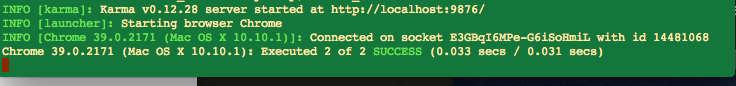
\includegraphics[width=0.9\textwidth]{Billeder/Test/test_exampel.png}
	\vspace{-0.0cm}
	\caption{Test eksempel}
	\label{fig:test_eksempel}
\end{figure}

Alt setup til Jasmine gøres i karma.conf.js filen som ligger i roden af projektet. Her bestemmes en række af opsætnings muligheder til frameworket. De mest væsentlige er følgende, hvilke filer Jasmine skal teste, hvilket output der ønskes til test, om testene skal køres en gang og derefter lukkes test programmet, eller om testene skal afvikles ved hvert gem af filer. 